\documentclass[12pt,aspectratio=169]{beamer}

\mode<presentation>
{
  \usetheme{Singapore}
 %\setbeamersize{text margin left=.6cm,text margin right=.6cm}
%  \setbeamertemplate{navigation symbols}{} % suppress nav bar
%  \setbeamercovered{transparent}
}
\usefonttheme{professionalfonts}
\usepackage{graphicx}
\usepackage{tikz}
\usepackage{amsmath}
\usepackage{mathpazo}
\usepackage[scaled]{helvet}
\usepackage{xcolor,colortbl}
\usepackage{siunitx}
\usepackage[siunitx]{circuitikz} % to draw circuits!

\sisetup{number-math-rm=\mathnormal}

\title{Class 15: Maxwell's Equations---Problem Solving}
\subtitle{AP Physics}
\author[TML]{Dr.\ Timothy Leung}
\institute{Olympiads School}
\date{March 2018}

\newcommand{\pic}[2]{\includegraphics[width=#1\textwidth]{#2}}
\newcommand{\mb}[1]{\mathbf{#1}}
\newcommand{\eq}[2]{\vspace{#1}{\Large\begin{displaymath}#2\end{displaymath}}}

\begin{document}

\begin{frame}
  \maketitle
\end{frame}

\begin{frame}
  \frametitle{Circuits}
  \begin{columns}
    \column{.25\textwidth}
    \begin{center}
      \vspace{-.2in}
      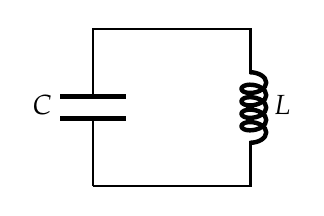
\begin{tikzpicture}
        \draw[thick](0,0) to[C=$C$](0,2)--(2,2) to[L=$L$] (2,0)--(0,0);
      \end{tikzpicture}
    \end{center}

    \column{.75\textwidth}
    An ideal circuit consists of a capacitor $C$ and inductor $L$. The capacitor
    is fully charged. The switch is closed at time $t=0$. Which of the following
    statements is true of the behavior of the circuit after the
    switch is closed?
  \end{columns}
  \begin{enumerate}[(a)]
  \item The capacitor will discharge through the inductor, and the current will
    decrease to zero.
  \item The capacitor will discharge through the inductor, transferring
    potential energy to kinetic energy.
  \item The capacitor will discharge through the inductor, transferring energy
    to the inductor, then the inductor will recharge the capacitor.
  \item The capacitor will discharge through the inductor, and the inductor
    will store the charge.
  \item The capacitor will not discharge through the inductor, so there will be
    no current.
  \end{enumerate}
\end{frame}



\begin{frame}
  \frametitle{Files for You to Download}
  Download from the school website:
  \begin{enumerate}
  \item\texttt{17-emReview.pdf}---This presentation. The slides only
    contain the problems that we are solving in class, but you will have to
    follow (and write) the solution yourself.
  \end{enumerate}
\end{frame}


\begin{frame}
  \frametitle{Maxwell's Equations}
  Which of the Maxwell's equations below indicates that there are no
  magnetic monopoles?
  \begin{enumerate}[(a)]
  \item $\displaystyle\int\mb{E}\cdot d\mb{A}=\frac{q}{\varepsilon_0}$
  \item $\displaystyle\int\mb{B}\cdot d\mb{A}=0$
  \item $\displaystyle\int\mb{B}\cdot d\mb{\ell}=\mu_0 I_{\textrm{inc}}$
  \item $\displaystyle\int\mathcal{E}=\mb{E}\cdot d\mb{\ell}=-\frac{d\Phi}{dt}$
  \item $\displaystyle\int\mb{g}\cdot d\mb{A}=-4\pi GM$
  \end{enumerate}
\end{frame}


\begin{frame}
  \frametitle{Maxwell's Equations}
  Which of the Maxwell's equations below relates electric flux to charge
  enclosed in a closed surface?
  \begin{enumerate}[(a)]
  \item $\displaystyle\int\mb{E}\cdot d\mb{A}=\frac{q}{\varepsilon_0}$
  \item $\displaystyle\int\mb{B}\cdot d\mb{A}=0$
  \item $\displaystyle\int\mb{B}\cdot d\mb{\ell}=\mu_0 I_{\textrm{inc}}$
  \item $\displaystyle\int\mathcal{E}=\mb{E}\cdot d\mb{\ell}=-\frac{d\Phi}{dt}$
  \item $\displaystyle\int\mb{g}\cdot d\mb{A}=-4\pi GM$
  \end{enumerate}
\end{frame}

\begin{frame}
  \frametitle{Maxwell's Equations}
  Which of the Maxwell's equations below relates the electric field
  produced to a changing magnetic flux?
  \begin{enumerate}[(a)]
  \item $\displaystyle\int\mb{E}\cdot d\mb{A}=\frac{q}{\varepsilon_0}$
  \item $\displaystyle\int\mb{B}\cdot d\mb{A}=0$
  \item $\displaystyle\int\mb{B}\cdot d\mb{\ell}=\mu_0 I_{\textrm{inc}}$
  \item $\displaystyle\int\mathcal{E}=\mb{E}\cdot d\mb{\ell}=-\frac{d\Phi}{dt}$
  \item $\displaystyle\int\mb{g}\cdot d\mb{A}=-4\pi GM$
  \end{enumerate}
\end{frame}

\end{document}

